\documentclass[12pt,compress,ngerman,utf8,t]{beamer}
\usepackage{etex}
\usepackage[ngerman]{babel}
\usepackage{graphicx}
\usepackage[export]{adjustbox}
\usepackage{multicol}


\usetheme[numbering=fraction, progressbar=frametitle]{metropolis}


\date{\today}
\institute{University of Freiburg}
\titlegraphic{\hspace{9cm} 
\includegraphics[height=2cm]{template/Logo-Uni-Freiburg.png}}
\graphicspath{ {./template/} {./strategy/} }

\title{Strategie}
\author{Felix Karg}
\subject{Mathecamp}

\newif\iffinal
\finaltrue
% \finalfalse

\AtBeginSection[]
{
    \begin{frame}{Inhalt}
        \begin{multicols}{2}
            \small
            \tableofcontents[currentsection]
        \end{multicols}
        \clearpage
    \end{frame}
}

\AtBeginSubsection[]
{
    \small
    \begin{frame}{Inhalt}
        \begin{multicols}{2}
            \small
            \tableofcontents[currentsection,currentsubsection]
        \end{multicols}
        \clearpage
    \end{frame}
}

% \vspace{0.1cm}

\begin{document}

\maketitle

% multicols from:
% https://tex.stackexchange.com/questions/24343/splitting-toc-into-two-columns-on-single-frame-in-beamer

\begin{frame}{Inhalt}
    \small
    \begin{multicols}{2}
        \small
        \tableofcontents[hidesubsections]
    \end{multicols}
    \clearpage
\end{frame}


% \section{Recap}



\begin{frame}[c]{}
    \center
    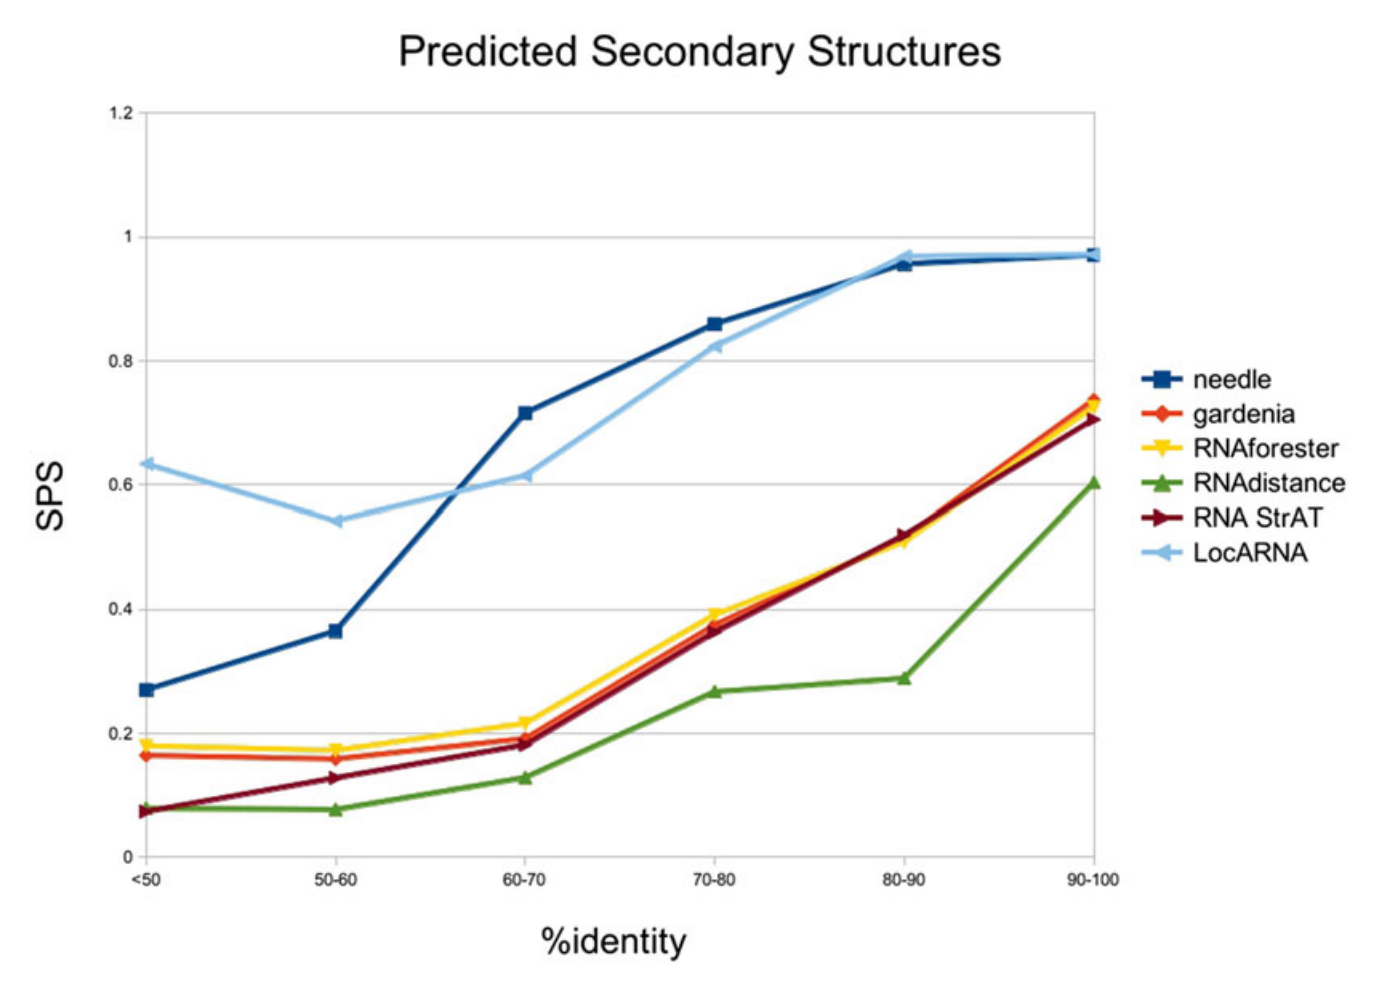
\includegraphics[width=\textwidth]{predicted}
\end{frame}


\begin{frame}[c]{}
    \center
    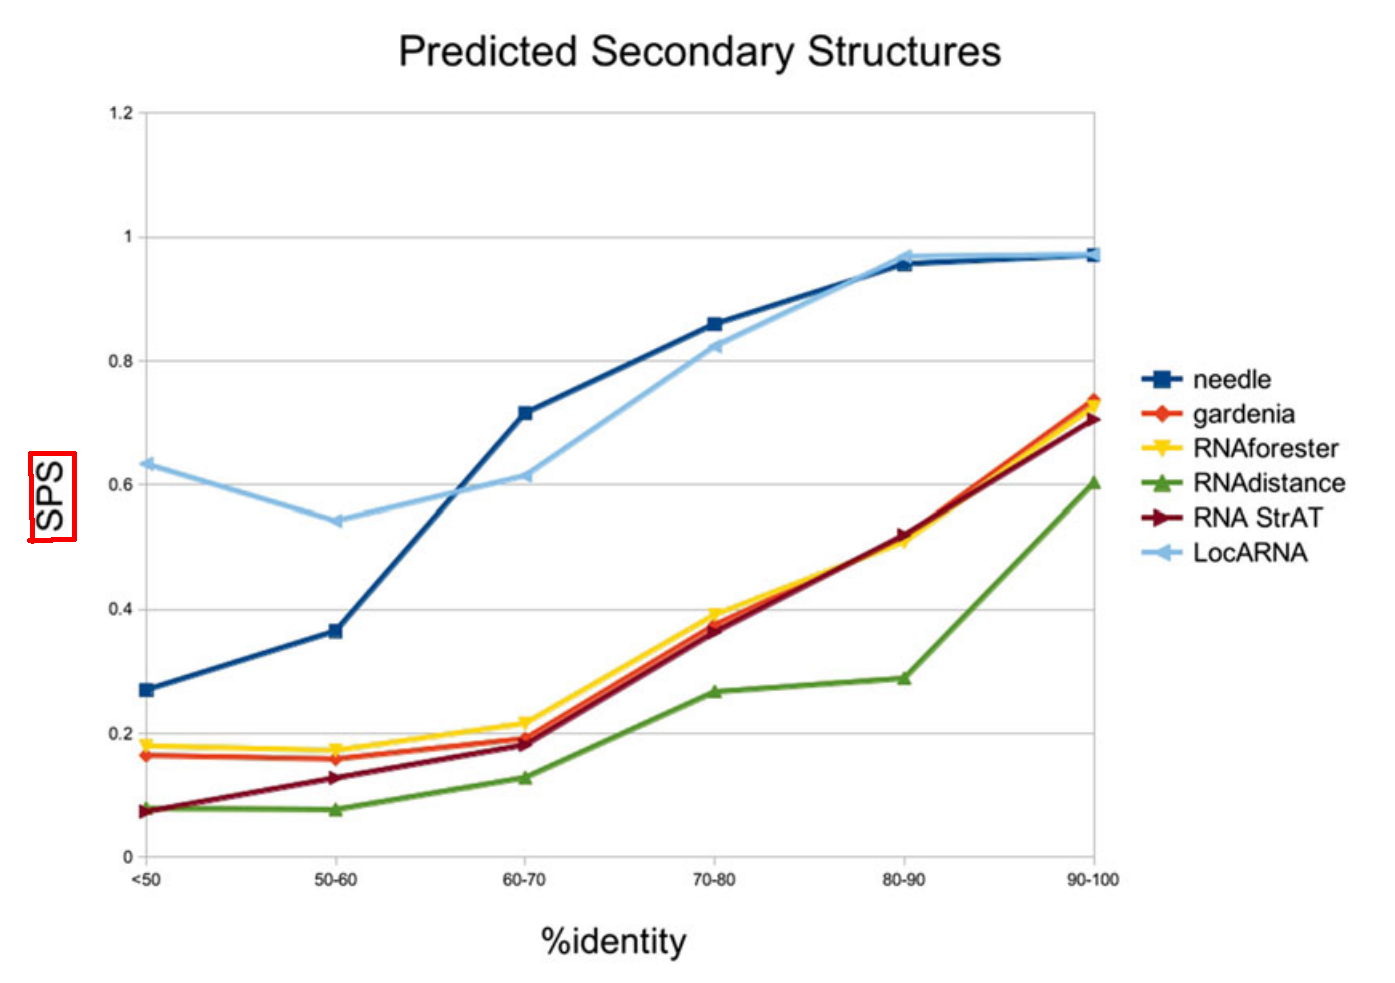
\includegraphics[width=\textwidth]{predicted_sps}
\end{frame}


\begin{frame}[c]{SPS - introduction}
    Sum of Pairs Score
    \newline
%    \vspace{2cm}
    \newline
    \pause
    Used to measure the \only<2-2>{alignment}\only<3->{similiarity} of two RNA sequences
\end{frame}


\begin{frame}[c]{Sequence Similiarity - Example}
    A: \only<4-5>{AAGGC}\only<1-1>{AAGGC}\only<2-3>{{\color{ForestGreen} AAGGC}}\only<1,4->{TT}\only<2-3>{{\color{red}TT}} \\
    B: \only<1-1>{AAGGC}\only<2-5>{{\color{ForestGreen} AAGGC}} \\
    C: \only<1-3>{AAGGC}\only<4->{{\color{ForestGreen} AAGGC}}\only<4-5>{{\color{red}AT}}\only<-3>{AT} \newline
    \newline
    Similiarity: \only<3,5>{60\% = 1 - (2 / 5) } \\
    1 - (edit distance / unaligned length of shorter sequence)
\end{frame}


\begin{frame}[c]{Sequence Similiarity - Example}
    A: {\color{ForestGreen}AAGGC}{\color{red}T}{\color{ForestGreen}T} \\
    B: AAGGC \\
    C: {\color{ForestGreen}AAGGC}{\color{red}A}{\color{ForestGreen}T} \newline
    \newline
    Similiarity: \only<2>{ 86\% = 1 - (1 / 7) } \\
    1 - (edit distance / unaligned length of shorter sequence)
\end{frame}


\begin{frame}[c]{}
    \center
    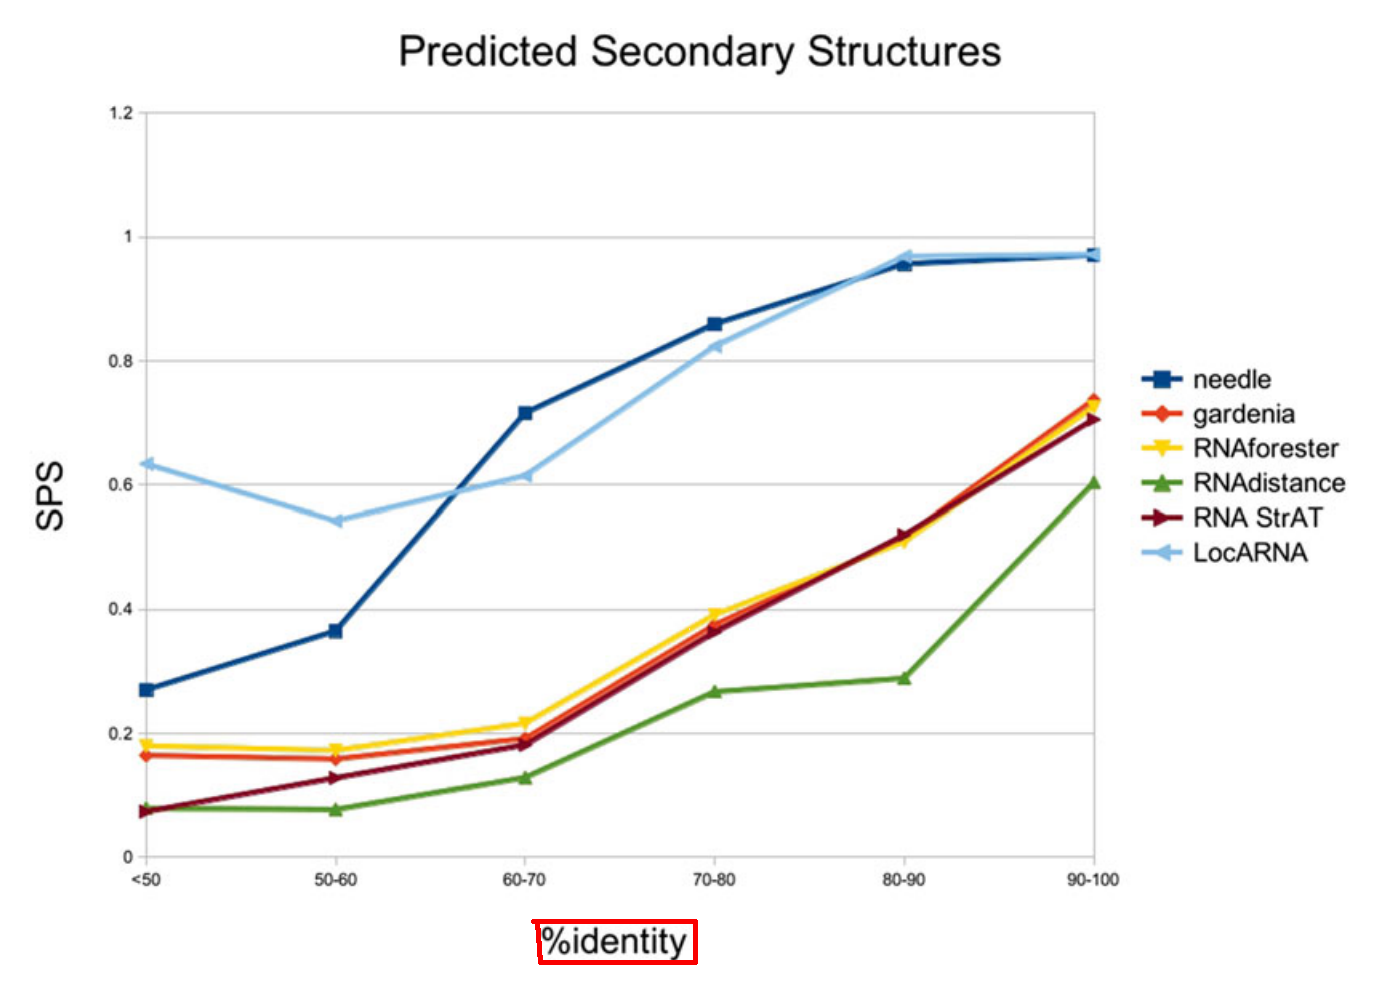
\includegraphics[width=\textwidth]{predicted_identity}
\end{frame}


\begin{frame}[c]{Sequence Identity - Example}
    A: \only<4-5>{AAGGC}\only<1-1>{AAGGC}\only<2-3>{{\color{ForestGreen} AAGGC}}TT \\
    B: \only<1-1>{AAGGC}\only<2-5>{{\color{ForestGreen} AAGGC}} \\
    C: \only<1-3>{AAGGC}\only<4-5>{{\color{ForestGreen} AAGGC}}AT \newline
    \newline
    Identity: \only<3,5>{100\%} \\
    Identical nucleotides / shorter sequence length
\end{frame}


\begin{frame}[c]{Sequence Identity - Example}
    A: {\color{ForestGreen}AAGGC}{\color{red}T}{\color{ForestGreen}T} \\
    B: AAGGC \\
    C: {\color{ForestGreen}AAGGC}{\color{red}A}{\color{ForestGreen}T} \newline
    \newline
    Identity: \only<2>{85\% = 6 / 7} \\
    Identical nucleotides / shorter sequence length
\end{frame}


\begin{frame}[c]{needle}
    \center
    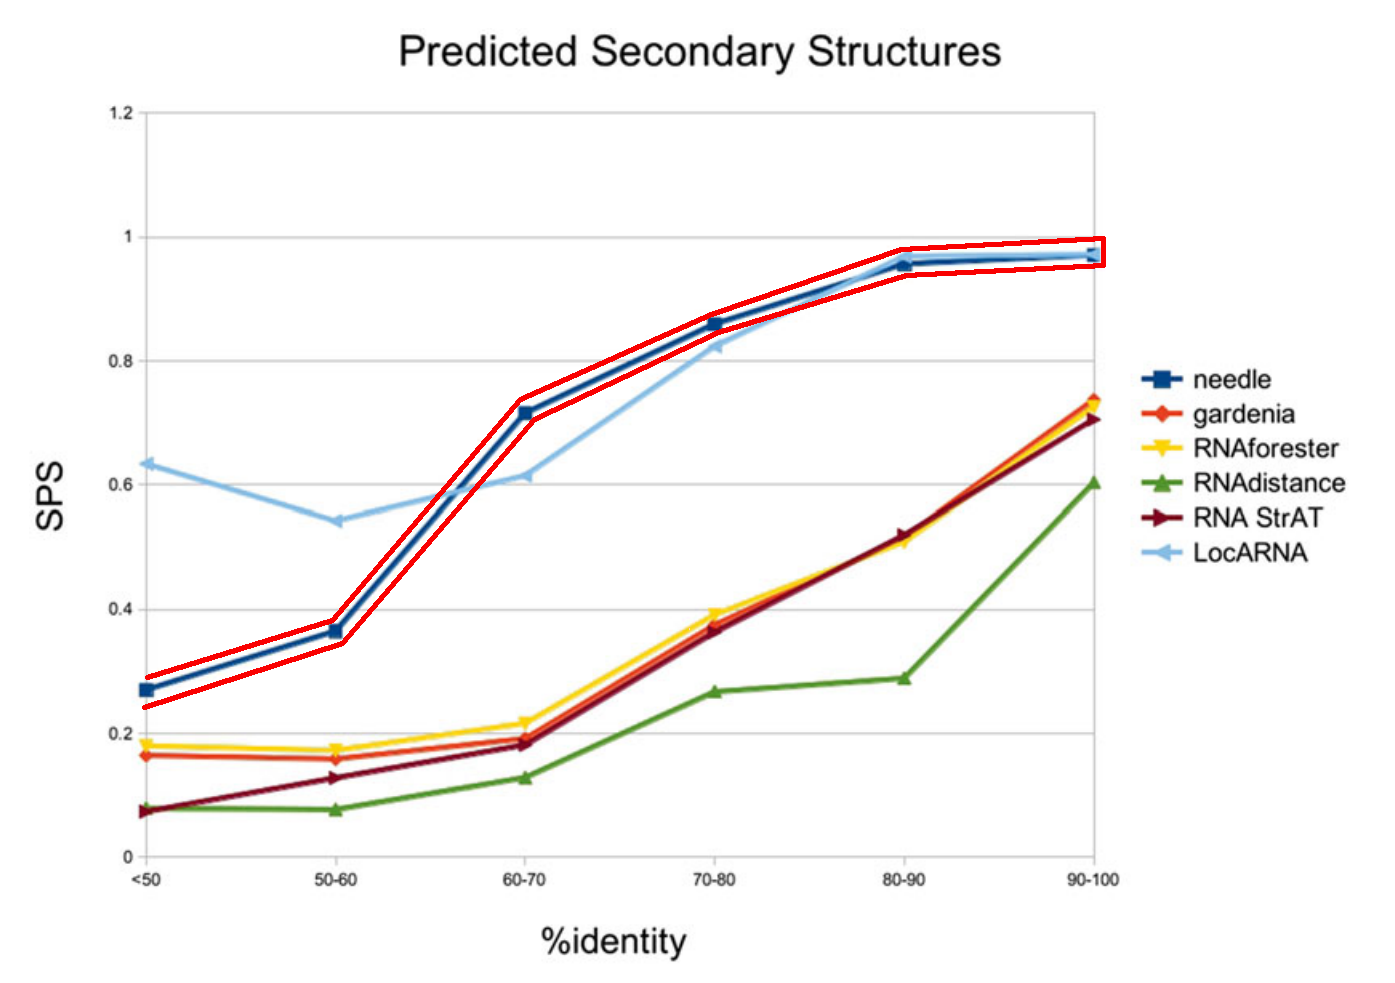
\includegraphics[width=\textwidth]{predicted_needle}
\end{frame}

\begin{frame}[c]{Needleman-Wunsch-Algorithm}
    \center
    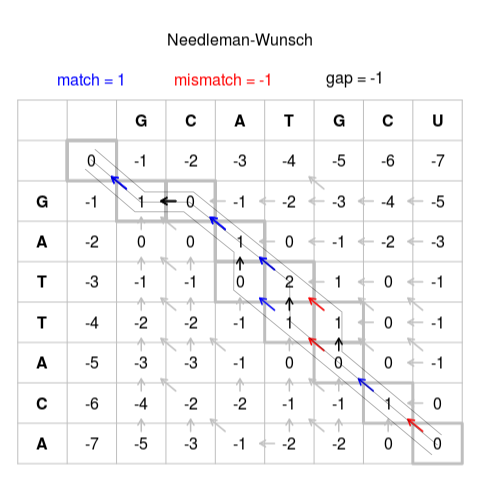
\includegraphics[width=0.75\textwidth]{Needleman-Wunsch_pairwise_sequence_alignment}
\end{frame}













% now %



%%%%%%%%%%%%%%%%%%%%%%%%%%%%%%%%%%%%%%%%%%%%%%%%%%SECTION%%%%%%%%%%%%%%%%%%%%%%%%%%%%%%%%%%%%%%%%%%%%%%%%%%
\section{Analyse}
%%%%%%%%%%%%%%%%%%%%%%%%%%%%%%%%%%%%%%%%%%%%%%%%%%SECTION%%%%%%%%%%%%%%%%%%%%%%%%%%%%%%%%%%%%%%%%%%%%%%%%%%

\begin{frame}{Analyse I - Finden versteckter Stärken}
    % Mehrere Optionen:
    %   Wal-Mart (?)
    %   David & Goliath (?) (Melly fragen!)
    %   Dosen-Abfüll-Dings (?!)
\end{frame}




%%%%%%%%%%%%%%%%%%%%%%%%%%%%%%%%%%%%%%%%%%%%%%%%%%SECTION%%%%%%%%%%%%%%%%%%%%%%%%%%%%%%%%%%%%%%%%%%%%%%%%%%
\section{Echte Strategie}
%%%%%%%%%%%%%%%%%%%%%%%%%%%%%%%%%%%%%%%%%%%%%%%%%%SECTION%%%%%%%%%%%%%%%%%%%%%%%%%%%%%%%%%%%%%%%%%%%%%%%%%%
\subsection{Kernelemente echter Strategie}
\subsection{Sich einen Vorteil verschaffen}
\subsection{Fokus}
\subsection{Design}
\subsection{Einen Vorteil verwenden}



% 



%%%%%%%%%%%%%%%%%%%%%%%%%%%%%%%%%%%%%%%%%%%%%%%%%%SECTION%%%%%%%%%%%%%%%%%%%%%%%%%%%%%%%%%%%%%%%%%%%%%%%%%%
\section{Beispiele für Gute Strategie}
%%%%%%%%%%%%%%%%%%%%%%%%%%%%%%%%%%%%%%%%%%%%%%%%%%SECTION%%%%%%%%%%%%%%%%%%%%%%%%%%%%%%%%%%%%%%%%%%%%%%%%%%

\begin{frame}{Reminder: Gute Strategie}
    Gute Strategie besteht aus:
    \begin{itemize}
        \item Einer Leit-Idee
        \item Einem Ziel
        \item Einem Plan an Kohärenten Aktionen, um zu diesem Ziel zu gelangen
    \end{itemize}
\end{frame}

\begin{frame}[c]{Gute Strategie: Beispiel Intel}
    Intel hat einiges Richtig gemacht:
    \begin{itemize}
        \item War ursprünglich Arbeitsspeicher-Hersteller \pause
        \item Radikaler Umschwung z
    \end{itemize}
\end{frame}



\begin{frame}[c]{Gute Strategie: Beispiel SpaceX}
    Wie sah die Raumfahrt-Industrie vor SpaceX aus? \pause


    Es gab:
    \begin{itemize}
        \item die ULA (United Launch Alliance)
        \item Arianespace (ESA-basiert)
        \item Das Russische Kommerzielle Programm
        \item (Das Chinesische und Japanische Raumfahrt-Programm)
    \end{itemize}

\end{frame}



\begin{frame}[c]{Raketen}

    \begin{tabular}{l|l|l|l|l}
        Wer &   Rakete         &   zum LEO &  zum GTO  &  Kosten         \\ \hline
        ULA & Delta IV (Heavy) & 22'560 Kg & 13'400 Kg & 400 Mio \$      \\ \hline
        ULA & Atlas V          & 18'510 Kg &  8'900 Kg & 150 Mio \$      \\ \hline
        ESA & Ariane 5         & 20'000 Kg & 10'500 Kg & 220 Mio \$      \\ \hline
        ESA & Soyuz II         &  8'200 Kg &  3'250 Kg & 60 Mio  \$      \\ \hline
        ILS & Proton-M         & 23'000 Kg &  6'920 Kg & 150 Mio \$      \\
    \end{tabular}


    \footnotesize
    Disclaimer: es ist sehr Schwer Korrekte Preis-Angaben zu finden, da diese meist nicht Öffentlich sind.
    Auch die Traglasten sind nicht exakt Angebbar, da ständig irgendwelche Verbesserungen (zumindest in letzter Zeit)
    gemacht werden.

\end{frame}


\begin{frame}[c]{SpaceX}

    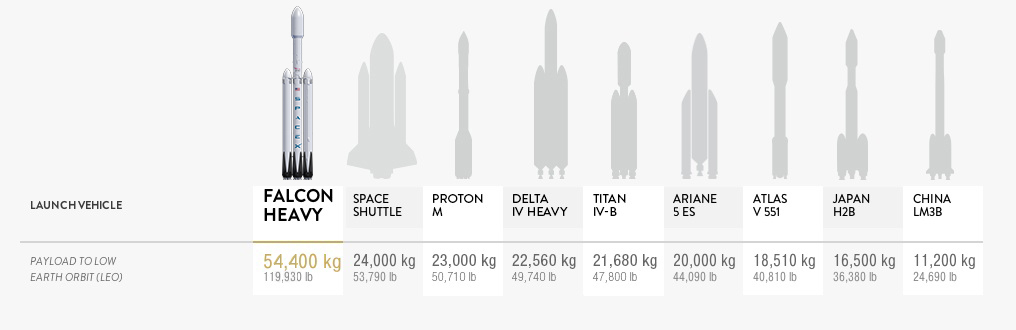
\includegraphics[height=3cm]{comparison.jpg} \\

    \begin{tabular}{l|l|l|l|l}
        Rakete       & zum LEO   & zum GTO   & Traglast zum Mars & Kosten \\ \hline
        Falcon 9     & 22'000 Kg &  8'300 Kg &  4'200 Kg         & 60Mio  \\ \hline
        Falcon Heavy & 54'400 Kg & 22'200 Kg & 13'400 Kg         & 90Mio  \\
    \end{tabular}


    \footnotesize
    Unter der Annahme, dass die Booster / Erste Stufe nicht wiederverwendet wird.
    Andernfalls sind ca. 30\% der Traglast abzuziehen

\end{frame}


%%%%%%%%%%%%%%%%%%%%%%%%%%%%%%%%%%%%%%%%%%%%%%%%%%SECTION%%%%%%%%%%%%%%%%%%%%%%%%%%%%%%%%%%%%%%%%%%%%%%%%%%
\section{Quellen}
%%%%%%%%%%%%%%%%%%%%%%%%%%%%%%%%%%%%%%%%%%%%%%%%%%SECTION%%%%%%%%%%%%%%%%%%%%%%%%%%%%%%%%%%%%%%%%%%%%%%%%%%
\begin{frame}[c,fragile,allowframebreaks]{Quellen}
    Die Folien sind zu finden unter: \\
    \url{https://github.com/fkarg/things-to-talk-about/tree/master/strategy}


    Das Buch, aus dem ich den Vortrag gebastelt hab:

    \begin{thebibliography}{10}
    \beamertemplatebookbibitems
    \bibitem{Richard Rumelt}
        Richard Rumelt
        \newblock {\em Good Strategy / Bad Strategy}.
        \newblock The Difference and Why It Matters \\
                  ISBN: 978-1-78125-154-6
    \beamertemplatearticlebibitems
    \bibitem{Wikipedia}
        Wikipedia
            \newblock {\em Battle of Trafalgar}
            \newblock \url{https://en.wikipedia.org/wiki/Battle\_of\_Trafalgar}
    \bibitem{Wikipedia}
        Wikipedia
            \newblock {\em SpaceX}
            \newblock \url{http://www.spacex.com/}
    \bibitem{Wihipedia}
        Wikipedia
            \newblock {\em Proton-M}
            \newblock \url{https://en.wikipedia.org/wiki/Proton-M}
    \bibitem{Wikipedia}
        Wikipedia
            \newblock {\em Ariane 5}
            \newblock \url{https://en.wikipedia.org/wiki/Ariane\_5}
    \bibitem{Wikipedia}
        Wikipedia
            \newblock {\em Delta IV Heavy}
            \newblock \url{https://en.wikipedia.org/wiki/Delta\_IV}
    \end{thebibliography}
    % required the allowframebreaks for longer lists

\end{frame}





\end{document}
